\chapter{Interpolation}

\section{Linear Interpolation}

  \begin{align}
    \lerp\left( A, B, t \right)
    &= \left( 1 - t \right) A + tB \\
    &= A + t\left( B - A \right)
  \end{align}

  \begin{itemize}
    \item $ A $: start
    \item $ B $: target
    \item $ t $: time
  \end{itemize}

\section{Spherical Interpolation}

  Spherical interpolation interpolate quaternions on a sphere

  \begin{align}
    \theta &= \cos^{-1}\left( a \cdot b \right) \\
    \slerp\left( t, a, b \right) &=
      \frac{\sin\left( \left( 1 - t \right) \theta \right)}{\sin \theta} a
      + \frac{\sin\left( t \theta \right)}{\sin \theta} b
  \end{align}

  \begin{figure}[H]
    \centering
    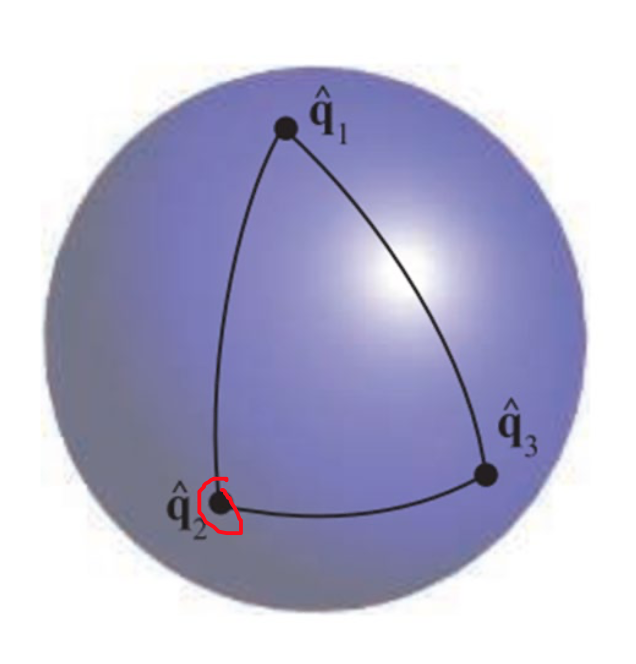
\includegraphics[width=0.2\columnwidth]{images/interpolation/slerp-jerk.png}
  \end{figure}

  Spherical interpolation, $ \vec{q_{1}} \to \vec{q_{2}} \to \vec{q_{3}} $,
  would experience a jerk during midpoint $ \vec{q_{2}} $

\section{Squad Interpolation}

  Squad interpolation is slerp with control points ($ a $) to pull the path
  away from jerk points

  \begin{equation}
    a_{i} =
      q_{i} \exp
      \left(
        - \frac{\log\left( q_{i}^{-1} q_{i - 1} \right)
        + \log\left( q_{i}^{-1} q_{i + 1} \right)}{4}
      \right)
  \end{equation}

  \begin{multline}
    \squad\left( q_{i}, q_{i + 1}, a_{i}, a_{i + 1}, t \right) = \\
      \slerp\left(
        \slerp\left( q_{i}, q_{i + 1}, t \right),
        \slerp\left( a_{i}, a_{i + 1}, t \right),
        2t \left( 1 - t \right)
      \right)
  \end{multline}

  Won’t actually overlap the control points; the control points pull the
  interpolation to avoid the jerk
